\documentclass[11pt]{book}

\usepackage{graphicx}
\usepackage{eso-pic}
\usepackage{tcolorbox}
\usepackage{polyglossia}
\setdefaultlanguage[indentfirst=false,forceheadingpunctuation=false]{russian}
\setotherlanguages{english}

\RequirePackage[a4paper, headsep = 0.5 \headsep, left=2.5cm, right=2.1cm, top=2cm, bottom=2.1cm]{geometry}

\setmainfont{Times New Roman}
\newfontfamily\cyrillicfont{Times New Roman}[Script=Cyrillic, Ligatures=TeX]

\usepackage{enumitem}
\setlist[itemize, 1]{label =\raisebox{-0.3\height}{\scalebox{1.8}{\textbullet}}}

\title{Философия эмоций}
\author{Кристина Тапполет}
\date{2023}
\begin{document}

\AddToShipoutPictureBG*{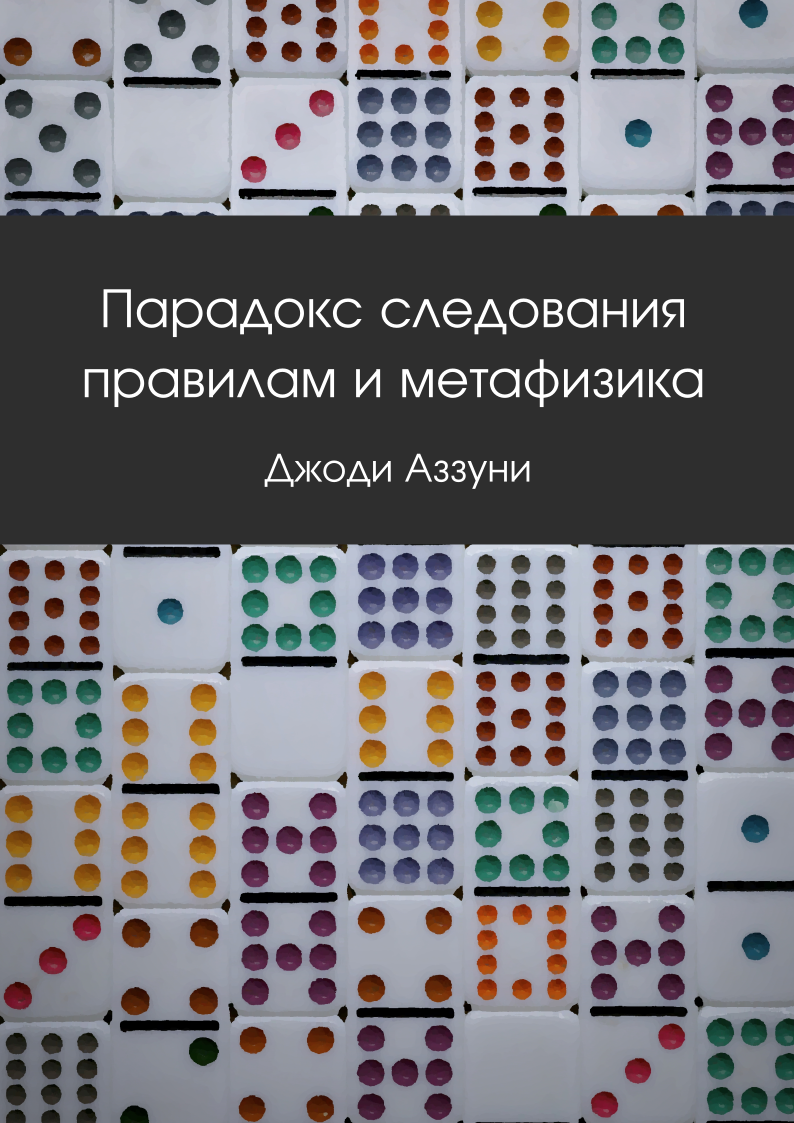
\includegraphics[width=\paperwidth]{title.png}}

\null
    \thispagestyle{empty}%
    \addtocounter{page}{-1}%
    \newpage

\tableofcontents

\part{Философия и наука об эмоциях}

\chapter{Философия эмоций}

\section{Введение}

Представьте, что пытаетесь набирать текст будучи запертым в иглу, и ''комок слякоти из перегретого купола уже в третий раз падает в пишущую машинку, заканчивая вашу работу на сегодня'' (Бриггс 1970, 259). Фрустрация и гнев в такой ситуации вполне понятны. Но антрополог Джин Л. Бриггс обнаружила, что понятны они не для всех --- в своей книге ''Без гнева'' (1970) она описывает эмоциональную жизнь уткухихалингмиутов (утку, для краткости) --- общины инуитов в арктической тундре к северо-западу от Гудзонова залива, где она провела полтора года. На собственном горьком опыте она узнала, что утку выражают неодобрение остракизмом --- им запрещается злится. Конечно, к вспышкам гнева у детей они терпимы, но взрослые должны контролировать свои эмоции. Потому злость, а вместе с ней грусть и любовь они выражают куда реже, чем это делается, скажем, в средней североамериканской семье. Казалось бы --- печальный факт, но в их суровой природной среде жесткий контроль сильных эмоций и сопровождающего их насилия вполне оправдан.

Подобные нормы есть и в других культурах --- идеал жизни, лишенной эмоциональных потрясений многим показался привлекательным. Например, согласно Стоицизму, страх, гнев и зависть --- иррациональные импульсы, связанные с ложными суждениями, и от эмоций, значит, нужно освободиться, чтобы достичь спокойствия ума. Буддизм также призывает отказаться от ненависти, и даже от желания и любви --- состояний, влекущих привязанности, удерживающие от освобождения. Да и в современных обществах к эмоциям относятся как минимум с осторожностью --- страх, гнев, зависть, отвращения и даже сострадание или любовь, считается, мешают ясно мыслить.

Но указывается также, что эмоции могут быть и полезны --- страх помогает избежать опасности, отвращение --- употребления вредных веществ. Иногда мы даже стремимся испытать негативные эмоции без, казалось бы, какой-то пользы: прыгаем с парашютом, слушаем грустную музыку или смотрим фильмы ужасов. А гнев помогает справиться с противником, и иногда кажется оправданным --- ''праведным гневом''. Уж тем более трудно отрицать пользу положительных эмоций --- сострадания, любви, радости, восхищения и надежды --- к ним и удовольствию от них мы обычно стремимся, и они, похоже, ключевой компонент счастливой жизни. Принято считать, что жизнь, лишенная эмоций --- и положительных, и отрицательных --- была бы бедна и едва ли человечна. Кто бы выбрал таковую жизнь андроида Дейты из ''Звездного пути'' --- владеющего мощнейшим позитронным мозгом, но вовсе не испытывающего эмоции?

Итак, наше отношение к эмоциям неоднозначно --- кажется, что следует быть не слишком им подверженным, и все же хочется вести полноценную, наполненную ими, жизнь. Эта амбивалентность проявляется не только в противоположных оценках эмоций, но и, собственно, эмоционально --- мы боимся гнева, отвращения, любви, и самого страха порой тоже боимся. И все же эти переживания нас привлекают --- и позитивные, такие как любовь и радость, и негативные, такие как гнев и страх. Но так думают большинство людей независимо от жизненного уклада и профессии, а что насчет философов? Конечно, философы тоже люди, и чувства их не могут принципиально отличаться. Так что и мысли их по поводу эмоций не отличаются фундаментально.

Чтобы дать представление о деятельности философов в этом направлении, я сделаю краткий исторический обзор философии эмоций. Обзор этот, конечно, избирателен и фокусируется лишь на нескольких основополагающих фигурах, тем самым игнорируя, быть может, не менее значительных --- Баруха Спинозу (1632-1677) и Адама Смита (1723-1780), например, а также не-европейских мыслителей --- таких как конфуцианский философ Мэн-Цзы (ок. 1040-221 гг. до н.э.) (Мэн-Цзы 2008, см. Вираг 2017; Ван Норден 2019; Вонг 2019) или буддийский философ Буддхагхоша (V-ый век) (Буддхагхоша 1984, см. Хейм 2013, Таске 2016), не говоря уже о женщинах-мыслителях, которым не предоставилась возможность оставить след в истории идей (см. Суперсон 2020).

\section{Эмоции: от Платона до Фомы Аквинского}

Современная западная философия берет свое начало в Древней Греции, и философия эмоций не исключение. И хотя ни Платон (ок. 429-347 гг. до н.э.), ни Аристотель (384-322 гг. до н.э.) не разработали законченную теорию эмоций (или страстей --- \textit{pathê} --- того, что мы претерпеваем, будучи по отношению к нему пассивны), они придерживались особых на них взглядов, оказавших огромное влияние --- и продолжающих влиять --- на мыслителей и по сей день (см. Прайс 2009). Оба они --- и Платон, и Аристотель --- считали человеческий разум (или ''душу'' --- \textit{psyche}) разделенным на части. Согласно ''Государству'' Платона, душа состоит из рациональной части --- разума, и низшей, нерациональной, делящейся на яростную (тумос) и страстную (эпитумия). Яростная часть ответственна за гнев, стыд, негодование, страх, гордость и восхищение, а страстная связана с телесными желаниями, такими как жажда и голод. Можно подумать, что эмоций касается только яростная часть --- но нет --- и Платон прямо утверждал, что эмоции сопровождают и некоторые телесные желания. Более того, он относил любовь к истине и мудрости к разумной части. Примечательно, что, согласно Платону, эмоции --- не исключительно психическое явление --- и они, и телесные позывы, он считал, соответствуют телесным нарушениям. Так, гнев, например, сопровождается кипением крови от мысли о несправедливости.

Центральное место в концепции души Платона занимает возможность конфликта между разными ее частями. Например, особый недостаток рациональности, называемый акрасией (слабость воли), Платон определял как совершаемое несмотря на веру в его неправильность, и объяснял в терминах конфликта между страстной и рациональной установкой. И чтобы таких конфликтов не было, рациональная часть, конечно, должна преобладать --- в ''Федре'' он сравнивает разум с возничим, ведущим двух тянущих в разные стороны крылатых коней. Платон, впрочем, считал яростную часть ближе и податливей разуму (в сравнении со страстной) и допускал возможность научиться, например, любить и ненавидеть так, чтобы конфликта с разумом не возникало.

У Аристотеля была схожая иерархия в его концепции, только он делил душу на две части: рациональную и не-рациональную --- ответственную за эмоции. В ''Никомаховой этике'' он включает в список эмоций телесные желания (эпитумию), а также гнев, страх, уверенность, зависть, радость, любовь, ненависть, тоску, соперничество и жалость. Как и Платон, Аристотель говорит об эмоциях как о затрагивающих не только душу, но и тело, описывая разгневанного при мысли об оскорблении как вскипающего. Он дает определения ряда эмоций, среди которых гнев, негодование, стыд, жалость, зависть и страх. Гнев --- это желание мести, сопровождающееся болью из-за действительного или воображаемого пренебрежения к себе или близкому. Примечательно, что для гнева характерна не только боль, но и удовольствие [предвкушения мести]. Эмоции, считал Аристотель, включают боль или удовольствие, оценку (например, веру в незначительность чего-то или его опасность), мотивацию, а также телесные изменения.

Как и Платон, Аристотель указывал на эмоции как на частый источник иррациональности --- конфликт между ними и разумом может привести к действию вопреки здравому смыслу --- акрасии. Но он также признавал за эмоциями возможность играть положительную роль --- считал их ключевыми для моральных/этических добродетелей и счастья. Моральные добродетели --- привычки, тесно связанные с ощущением нужных эмоций в нужное время по отношению к нужным предметам и людям (см. главу 10), так что и гнев может быть правильной реакцией. Добродетели, считал Аристотель, требуют воспитания, и эмоциональные реакции зависят от паттернов, усвоенных в общественных взаимодействиях. Как становятся хорошими игроками на лире, тренируясь на ней играть, так и становятся храбрыми, встречаясь лицом с опасностью и приучаясь испытывать при этом правильные эмоции. Идея воспитания эмоций оказалась, вообще очень влиятельной (см. главу 12).

Аристотель считал эмоции необходимыми для добродетели и счастья --- но в рамках Стоицизма, важной школе мысли, основанной в Афинах в III веке до нашей эра и просуществовавшей вплоть до римского периода, к эмоциям относились куда более критично. В работах стоиков можно найти подробное рассмотрение таких негативных эмоций как гнев, страх, горе, печаль, стыд, зависть, ревность и жалость. В отличие от Платона и Аристотеля, они не верили в разделенную душу, представляя ее как физическую субстанцию (пневму), смешанную с телом. Душа, однако, обладает управляющей способностью, через которую реализуется, среди прочего, способность к рассуждению. Эмоции же --- согласно стоикам --- иррациональны, их надо не просто контролировать, но --- в идеале --- полностью искоренить. Согласно Сенеке (ок. 1 до н.э. - 65 н.э.), ''Гнев следует не контролировать, но совершенно уничтожить, ибо какой контроль возможен на по сети своей злобным?'' (Сенека, ''О гневе'', iii. 42). То есть разделяя душу на части, стоики не согласовывали, но противопоставляли их. Наличие эмоций --- источник акрасии, влекущей скорые и разрушительные изменения в душе.

Что же не так с эмоциями, согласно стоикам? Эмоции подразумевают суждения о добре и зле, которые глубоко ошибочны. Горе, например, следствие убеждения в действительном наличии нечта плохого --- согласие с наличием такого и заставляет считать реакцию правильной. Однако такого рода убеждения основаны на ошибочном представлении о человеке и его месте в мире. Хороша же только добродетель, и только соответствующие ей действия обеспечивают истинное счастье. Считать же важным что-нибудь еще --- свою удовольствие или боль, например --- не просто плохо, но иррационально, ведь ни к чему кроме несчастья это не приведет. Стоики предлагали разные методы избавления от эмоций --- от когнитивной терапии, включающей философские рассуждения, до развития соответствующих привычек и даже музыкальной терапии.

Стоиков часто высмеивали за их идеал --- существо, начисто лишенное эмоций, кажется недосягаемым для нормальных людей, но, справедливости ради, стоики и не рекомендовали жизнь, лишенную даже намека на эмоции. Допустимо чувствовать своего рода протоэмоциональную реакцию --- не соглашаясь с ней, не позволяя ей стать полноценной эмоцией, движущей к определенным действиям. Некоторые психические состояния, сейчас считаемые эмоциями, стоиками даже поощрялись --- например, восторг (если он вполне обоснован). Впрочем, даже с учетом этих уступок, идеал их может показаться чрезмерно требовательным и в целом нежелательным.

Средневековых философов тоже интересовали эмоции (их называли \textit{passio} или \textit{affectus}). Фома Аквинский (1225-1274), на подход которого значительно повлиял Аристотель, предложил наиболее обширную трактовку эмоций в своей ''Сумме теологии'' (Часть II -- 1.22--48 и 2.17--36) (см. Кнууттила 2004, Перлер 2018). Подобно стоикам, современники Фомы и он сам были сосредоточены на нормативном вопросе --- хороши или плохи эмоции, являются ли любовь, ненависть, надежда, отчаяние, страх, радость или гнев, добродетелью или грехом. Фома Аквинский, считавший эмоции движениями души, подчеркивал их побудительную силу. Эмоции --- это мотивация к действию: гнев, например --- желание мести. Мотивация эта связана с телесными изменениями и возникает из оценки чего-либо как приятного или болезненного или, вообще, значимого. Фома Аквинский называет эти категории ''формальными объектами'', и понятие это (как будет видно в Главе 2) до сих пор играет в философии эмоций важную роль. Поскольку оценки, на которых основаны эмоции, могут быть ошибочными, их, считал Фома, следует проверять разумом. Но искоренять эмоции не стоит --- достаточно держать их под контролем. Итак, Фома Аквинский следовал Аристотелю, утверждая необходимость для добродетели соответствующих разуму эмоций, и --- раз эмоции могут командам разума сопротивляться, контроль разума должен быть подобен политической власти над свободными сопротивляться. Рефлексия, считал он, способна не только ослабить, например, гнев, но и полностью его прекратить, и для этого достаточно помыслить вызывающее его в ином свете. Как будет видно из Главы 11, стратегия такой переоценки занимает центральное место в современных подходах к регуляции эмоций.

\section{Современная философия и эмоции}

Рене Декарт (1596-1650) (см. Шапиро 2020) обычно считается отцом современной философии. Декарт открыто презирал средневековые теории эмоций в своей книге ''Страсти души'' (1649/1989). Его занимала проблема отношения разума и тела, которые он считал отдельными субстанциями. Эмоции, согласно Декарту --- это восприятия, ощущения или волнения души, вызванные движениями животных духов --- мельчайших частиц, сообщающих душе готовность тела к определенным действиям. То есть эмоции затрагивают не только ум, но и тело. Примечательно, что животные (кроме человека), считал Декарт, не имеют разума и потому неспособны испытывать эмоции и даже просто чувствовать боль или удовольствие --- это резко контрастирует со взглядами его предшественников, допускающими способность животных испытывать эмоции даже не имея разума.

Но как взаимодействуют разум и тело? Это сложный вопрос, отвечая на который, Декарт разработал теорию, согласно которой, тело влияет на разум передачей своих движений посредством животных духов через шишковидную железу в основании мозга. Но эта теория, конечно, не может быть корректной --- если разум состоит из нефизической субстанции, то такой ''факс в душу'' не объясняет воздействие физического на разум.

Хотя Декарт и уделяет много внимания такому механистическому объяснению эмоций, его теория весьма схожа как с аристотелевской, так и со стоической. Так, говоря про эмоции как про волнения души, вызванные движением животных духов, он все же указывал, что некоторые из них включают оценку вещей с точки зрения вреда и пользы. Любовь и радость, например --- являясь одной из основных эмоций наряду с удивлением, ненавистью, желанием и печалью --- вызваны представлением своего объекта как хорошего и полезного[, при этом любовь, в отличие от радости подразумевает неизменность этих свойств со временем]. Эмоции обладают мотивационной силой и отличаются от оценочных суждений тем, что суждения требуют также активного согласия с оценкой. То есть можно выносить суждение о вещи как о хорошей, и все же невольно реагировать на нее как на плохую, не соглашаясь, впрочем, с этим представлением. Как будет видно в Главе 6, такие ''непокорные эмоции'' (Д'Армс и Джейкобсон, 2003) занимают видное место в современных дебатах о природе эмоций.

Декарт отличал эмоции от суждений еще тем, что эмоции могут вводить в заблуждение. Они часто искажают наше понимание реальности, заставляя верить, что все лучше или хуже, чем на самом деле, так что эмоции следует контролировать. Напрямую управлять эмоцией нельзя, но, считал Декарт, с первоначальной эмоциональной реакцией можно не соглашаться --- согласие же даст ей импульс к дальнейшему развитию. Косвенный контроль над эмоциями возможен посредством другой эмоции --- чувства собственного достоинства, способности свободно осуществлять свою волю. Декарт также выделял несколько способов изменить свои [первичные] эмоциональные реакции. Можно, во-первых, пытаться представить объект своих эмоций в ином свете. Или представить последствия эмоциональных реакций --- если они негативные, это будет постепенно притуплять порождающие их первичные реакции. В конце концов, частое столкновение с тем, что вызывает эмоциональные реакции, также постепенно притупляет их.

Другой известный философ этого периода --- Дэвид Юм (1711-1776) --- взял на себя задачу пересмотреть традиционную рационалистическую концепцию эмоций (см. Кохон 2018). Вместо поиска способов их контроля он прямо заявил, что эмоции играют --- и должны играть --- ведущую роль. В своем ''Трактате о человеческой природе'' он указал, что ''разум должен быть --- и был всегда --- только служанкой чувств'' (Юм 1739-1740/2000, Книга 2, Часть 3, Раздел 3). Роль разума --- полезная, но вспомогательная: он предоставляет информацию о мире и средствах к достижению наших целей, но цели эти предоставляются эмоциями. Разум сам по себе не обладает мотивационной силой и, значит, не в состоянии действительно противостоять эмоциям --- любая попытка такого мнимого противостояния предполагала бы своей причиной другие эмоции. В своем ''Трактате'' Юм утверждал, что эмоции не состоят в представлении вещей, а значит и не могут, подобно суждениям, оцениваться разумом как рациональные или иррациональные. Впрочем, в более поздней работе ''О стандарте вкуса'' (1757/1985a) Юм от этого тезиса отказался. Но в ''Трактате'' он также утверждал, что ''нет никакого противоречия в том, чтобы предпочесть смерть всего мира, царапине'' (Юм 1739-1740/2000, Книга 2, Часть 3, Раздел 3). Однако, Юм, конечно, решительно осудил бы такое предпочтение --- размышление о смерти мира вызывает ужас --- но рациональность или иррациональность здесь не при чем.

Юм выделяет два вида эмоций. Первый --- ''прямые страсти'' --- включает желание, отвращение, надежду, горе, радость, страх, отчаяние и противоположность страха --- чувство безопасности. Они вызываются соответствующим опытом или мыслью о добре и зле, что для Юма то же, что переживание удовольствия или боли или мысль о них. К так называемым же ''косвенным страстям'' относятся гордость, смирение, стыд, честолюбие, тщеславие, любовь, ненависть, зависть, жалость, злоба и щедрость --- помимо переживания боли или удовольствия, они требуют также дополнительных мыслей. Гордость за красоту своего дома, например --- удовольствие, направленное на самого себя и вызванное мыслью о принадлежности вам этого дома. Вообще, гордость соответствует положительному представлению о себе, а стыд --- отрицательному. То есть, согласно Юму, и прямые, и косвенные эмоции подразумевают оценку своих объектов, так что различие его теории с таковыми предшественников не так уж велико --- Юма отличает не столько описание природы эмоций, сколько понимание их взаимосвязи с разумом.

Такая инверсия отношения разума к эмоциям является ключевой для морального сентиментализма --- для Юма, моральные оценки берут свое начало из эмоций, а не из разума, и именно на основе удовольствия или неудовольствия в от восприятия людей и их действий, мы выносим моральные суждения. То есть добродетельным считается человек, характер которого вызывает одобрение, а одобрение --- это определенный род удовольствия. Удовольствие это опосредованно ''симпатией'' --- спонтанном ощущении удовольствия/неудовольствия при виде его у других. Так, доброжелательность одобряется потому что приносит удовольствие другим. Юм, как не странно, указывал на способность эмоциональных реакций вводить в заблуждение. Например, при рассмотрении личности врага мы склонны быть предвзятыми, из-за чего не можем дать ей справедливую оценку. Нам, значит, стоит принять нейтральную точку зрения, чтобы не допускать подобных отклонений.

Другой знаменитый философ --- Иммануил Кант (1724-1804) --- выступает против концепции морали Юма (см. Уилсон и Дэнис 2018). Юм указывал, что основание морали --- эмоции по отношению к другим, Кант же полагал ее основой практический разум --- способность определять волю и приводить к действию. Мораль, согласно Канту, возможна благодаря автономной воле --- той, что устанавливает сама себе закон. Такая воля должна игнорировать всякие привлекательные черты своих объектов, поскольку руководство ими значило бы руководство ''склонностями'', которые нам в действительности чужды. Следовать склонностям значило бы рабство --- такая воля не автономна. Поэтому эмоции не следует учитывать в принятии решения --- только так мы можем быть автономными агентами и соблюдать свои моральные обязательства.

Кант критиковал эмоции как основу для морали, указывая, что они слишком шатки для столь фундаментальной роли. В своей работе ''Основы метафизики морали'' (1785/1996) он утверждал, что такие ''эмпирические принципы'' не могут поддержать моральные законы, справедливые для всех [разумных] существ, ведь они привязаны к конкретной --- человеческой --- природе. Кант также отмечал ''бесконечные различия в степенях и видах чувств'', из-за чего они ''не могут предоставить единый стандарт хорошего и плохого'' (Кант 1785/1996, 4:442). Можно, впрочем --- независимо от вопроса об универсальности моральных принципов --- усомниться в справедливости такого осуждения эмоций, ведь наши рациональные способности так же зависят от нашей природы, а наши выводы могут различаться в разных обстоятельствах и даже сбивать нас с верного пути.

Кант, однако, не столь плохо относится к эмоциям, как можно было подумать. Так, одной конкретной эмоции --- уважению морального закона --- он отводит центральную роль. Эмоция эта возникает при рассмотрении морального закона и приводит к подчинению ему. Для таких существ, как мы, согласно Канту, требуется чувство удовольствия или восторга от выполнения своего долга. В более поздних работах (см., например, Кант 1797/2018) он даже указывал на обязанность культивировать такие моральные эмоции, как сострадание , любовь к людям и уважение к себе. В работе об эстетических суждениях Кант также отводил эмоциям центральную роль понимании красоты и возвышенного. И все же, в отличие от Юма, Кант считал подлинно моральными лишь действия, совершаемые исключительно из чувства долга.

Итак, видно, что интерес философов к эмоциям привел к появлению и развитию все более тонких и сложных их теорий. Но здесь имеет смысл задать вопрос: в чем, собственно, должно состоять философское исследование эмоций? Иначе говоря, какие основные вопросы предполагает эта область?

\section{Основные вопросы}

Большинство современных философов, конечно, сочли бы центральным философии эмоций вопрос ''Что такое эмоция?'' (выступающий также заголовком знаменитой статьи Уильяма Джеймса (1884)), и большая часть работы в этой области на нем и сосредоточена. Для ответа нужно разработать теорию, раскрывающую сущность эмоций, отделяющую их от прочих состояний, таких как зуд или мигрень, например. Многие философы прошлого (да и современные тоже) рассматривали эмоции как состоящие из нескольких компонентов. Так, согласно Аристотелю, они включают боль/удовольствие, оценки, мотивацию, а также телесные изменения. Есть ли среди этих компонентов те, что присущи всякой эмоции? Как вообще компоненты эмоций связаны друг с другом? Некоторые эмоции очень различаются --- страх и гордость, например --- так что имеет ли смысл говорить обо всех эмоциях сразу, или лучше рассмотреть только одну или две? Одна из задач философии эмоций --- выявить и объяснить различия между видами эмоций.

Впрочем --- и это видно из исторического очерка --- философов волнует не только вопрос о природе эмоций. Эмоции могут быть хороши или плохи, некоторые из них, значит, следует воспитывать, некоторые --- контролировать, от некоторых желательно вовсе отказаться (согласно стоикам --- почти от всех). Но даже радикальные критики эмоций соглашались, что есть эмоции, необходимые для счастья --- обоснованный восторг у стоиков и уважение к моральному у Канта, например. С другой стороны, даже те, кто отводил эмоциям главенствующие роли, отмечали вред от некоторых из них --- даже Юм признал, что эмоции могут приводить к ошибкам.

Такая двойственность в отношении эмоций --- признак их сложности: эмоции принимают самые разные формы и оттенки. Это также признак важности нормативного вопроса ''Хороши или плохи эмоции для нас?''. Иначе говоря, какова их функция? Из-за разнообразия эмоций, речь обычно заходит о нормативном статусе лишь нескольких или даже одной из них. Более того, обычно эмоция хороша в чем-то одном и плоха в другом: страх, например, помогает избежать опасности, но должен быть направлен на действительно опасный объект и быть не слишком сильным чтобы не перерасти в панику. Так или иначе, философы прошлого склонны были рассматривать эмоции именно с нормативной точки зрения.

Один из важных аспектов, рассматриваемых теориями эмоций --- их регулирование, будь то путем их воспитания, контроля или даже искоренения. Можно ли изменить наши эмоциональные реакции, и если да, то как? Такой вопрос, конечно, тесно связан с нормативным, ведь регулировать имеет смысл лишь то, что может быть хорошим или плохим. Более того, вопрос о природе эмоций можно рассматривать как инструментальный по отношению к вопросу их регулирования. Философы прошлого предоставили несколько способов такой регуляции, представляющих интерес не только для философов, но и для психологов.

Итак, философов [касательно эмоций] занимали три взаимосвязанных вопроса:

\smallskip

a) Вопрос о сущности: какова природа эмоций?

б) Нормативный вопрос: хороши или плохи эмоции [для нас]?

в) Вопрос регулирования: можем ли мы управлять эмоциями и если да, то как?

\smallskip

Наибольшее практическое значение имеет, конечно, нормативный вопрос, ведь от ответа на него зависит интерес к природе и регулированию эмоций. Конечно, остальные два вопроса тоже важны, и вопрос о природе --- наиболее фундаментальный. Зная, что такое эмоции, мы можем понять, как они могут быть плохи или хороши [для нас] и как мы можем --- если можем --- ими управлять. Вопрос же регулирования важен потому, что ответы на остальные два еще не способны дать практических рекомендаций.

До сих пор речь шла об интересах философов касательно эмоций, но они, конечно, не единственные, кого они занимают. Многие дисциплины --- от социальных наук до биологических наук, вносят свой вклад в понимание эмоций, не говоря уже об искусстве вообще и литературе в частности. В свете этого возникает вопрос о связи этих различных направлений друг с другом в рассмотрении эмоций.

\section{Актуальность результатов научных исследований}

Эмоции так или иначе изучаются очень многими научными дисциплинами, среди которых биология, психология, психиатрия, нейронауки, антропология, социология и история, а потому важна связь между этими разными к ним подходами. Проще говоря: как философам реагировать на результаты касательно эмоций из научных дисциплин? Должны ли философы передать тему эмоций социальным и биологическим так же, как передали биологии тему функционирования организмов? Или, может, философия способна выступить здесь интегратором результатов рассмотрения эмоций в разных их аспектах, предложив так единое их объяснение и, возможно, даже обнаружив недоступные в рамках отдельных дисциплин, выводы? Многие философы не согласны ни с первым, ни со вторым вариантом. Но что тогда может философия предложить в качестве особого подхода к эмоциям?

Во-первых, философия использует особые методы исследования эмоций. Во-вторых, ее интересуют другие касательно них вопросы. То есть у философов касательно эмоций есть и собственный предмет, и собственные методы (эту линию защиты см. в Робертс 2003). А значит, кажется, философам не обязательно уделять много внимания тому, что делается в прочих дисциплинах --- достаточно вежливого любопытства. Как же защитить эти два тезиса?

Начнем с методологического. Метафилософский вопрос о методах философии --- спорный, но большинство философов согласны, что основными инструментами являются концептуальный анализ, мысленные эксперименты, интроспекция и наблюдение. Но достаточно ли они точны и надежны? Во всяком случае, они сильно отличаются от экспериментальных и статистических методов, используемых в большинстве социальных и биологических наук. Даже философы, занимающиеся экспериментальной философией и использующие анкетирование, не используют микроскопы или сканеры МРТ. И все же, разрыв между философскими и научными методами не следует преувеличивать.

Возможно, научные методы не столь уж отличаются от философских, по крайней мере не так, как это кажется на первый взгляд. Научное наблюдение, конечно, гораздо систематичней любого используемого философами метода, но ведь и философии в той или иной мере свойственна систематичность. Интроспекция же может считаться своего рода наблюдением, что делает разрыв между философской и научной методологией еще меньше. Наконец, концептуальный анализ и мысленные эксперименты в некоторой мере необходимы и для научных исследований. Проверяемые гипотезы, пожалуй, невозможно представить без соответствующих концептуальных разъяснений, и в ходе разработки этих пояснений кажется необходимым рассмотреть примеры и контрпримеры. То есть различия между научным и философским методом --- если они есть --- касаются акцентов, и неясно, достаточно ли их для рассмотрения философского взгляда на эмоции как совершенно самостоятельного.

Эмоции --- сложное явление, а потому разные дисциплины изучают разные их аспекты. Нейронауки сосредоточены на нервной системе вообще и мозге в частности, и ищут основания эмоций в них; эволюционная биология рассматривает механизмы реагирования, которые помогли нашим предкам выжить и распространить свои гены; антропологию занимают социальные нормы, регулирующие эмоции, и т.д.. Из этого легко сделать вывод, что и у философии должен быть особый, интересующий только ее, аспект эмоций. Но давайте вернемся к трем центральным вопросам философии эмоций: имеет ли какой-нибудь из них исключительно философский характер?

Вопрос о сущности, казалось бы, только философов всегда и волновал. Разве сам термин ''сущность'' не сугубо философский? Однако используемая терминология может вводить здесь в заблуждение. Вопрос о сущности эмоций централен для философии эмоций, но представляет интерес и для прочих дисциплин. Ведь как, вообще, можно проводить эксперименты, посвященные эмоциям, не предполагая о них хоть что-то? Разные дисциплины предлагают разное понимание эмоций, по-разному их объясняя, так что вопрос о сущности не чисто философский.

Что же касается нормативного вопроса, то ученые часто относятся к таким вопросам с некоторой опаской, рассматривая их как сомнительные и даже ненаучные и способные заинтересовать только философов. Отчасти так оно и есть: вопросы о том, хороши эмоции для нас или плохи, --- это вопросы, занимавшие философов на протяжении веков, и философы, похоже, лучше всех к таким вопросам подготовлены, ведь этика является традиционной философской дисциплиной. Но прогресс в этих вопросах, очевидно, вряд ли возможен вне вклада из нефилософских дисциплин. Вопросом влияния эмоций на суждения, например, занимается психология, но они совершенно точно имеют отношение к пониманию влияния эмоций на моральный облик. Так же как и помощь эмоций в решении проблем должна быть подвергнута эмпирической, научной, оценке. Итак, нормативный вопрос, хотя и специфичен для философии, решаться должен с учетом результатов анализа эмпирических данных в рамках нефилософских дисциплин.

Аналогично дело обстоит с вопросом о регулировании эмоций. Он так же интересен не только философии --- им занимается психология, психиатрия и нейробиология. И философам, похоже, придется сотрудничать с учеными из этих дисциплин для эффективного его решения.

Итак, даже если нормативный вопрос специфичен для философии --- даже тогда для полноценного ответа на центральные вопросы философам нужно учитывать результаты из нефилософских дисциплин, и ни предполагаемые методологические различия, ни различные интересующие аспекты не гарантируют обратного. Подход, значит, должен быть междисциплинарным.

Здесь можно возразить, что даже включение философии в такой междисциплинарный подход не обязательно --- есть опасения касательно надежности ее инструментов. Возможно, стоит обойтись без них --- без, значит, концептуального анализа, мысленных экспериментов, интроспекции и обыденного наблюдения? Но они, похоже, в некоторой мере присущи и прочим дисциплинам, так что здесь нет однозначных причин отвергнуть философский подход.

В защиту философских методов скажу несколько слов о концептуальном анализе. Его основная идея в разбиений сложных концепций на простые с целью определения фундаментальных и построения уже из них новых сложных. Это схоже с химическим анализом, в рамках которого определяются фундаментальные химические элементы, из которых составлены сложные. Большинство обыденных понятий --- понятие знания, например --- сопротивляются такому анализу, и тогда зачастую лучше попытаться показать концептуальные связи между ними. Концептуальный анализ --- это важно --- не подразумевает редуцирование, \textit{сведение} одних концепций к другим, более фундаментальным. Концептуальные разъяснения позволяют выявить концептуальные истины, то есть утверждения, истинные в силу только лишь включаемых концепций. Желтый, например, является цветом, а то, что тяжелее слона, не может быть легче него. Или: если некто знает, что Земля круглая, то Земля круглая. Интересная особенность концептуальных истин --- направленность не на просто таки нейтральную регистрацию употребления терминов, а на понятия и мысли. Для разрешения противоречий между предполагаемыми концептуально истинными утверждениями и ответить на контрпримеры, нужен акт концептуального балансирования, в ходе которого некоторые утверждения также могут быть и отклонены.

Метод концептуального балансирования схож с методом рефлексивного равновесия, предложенным Джоном Ролзом в своей знаменитой работе ''Теория справедливости'' (1971). Ролз утверждал, что для получения обоснованных этических убеждений следует начать с некоторых приемлемых этических суждений и последовательно уточнять и исправлять их для получения теории. Аналогично, для получения концептуальных истин нужно начать с некоторых банальностей, непосредственно следующих из самих понятий и, сталкиваясь с противоречиями или контрпримерами, эти банальности корректировать --- модифицировать или отвергать --- постепенно получая все более связный их набор (Джексон 1998). Этот метод, как надеюсь продемонстрировать в следующих главах, успешно применим к связям между понятиями эмоций и оценочными понятиями.

Вообще, философское мышление может быть продуктивным в применении ко всем трем основным вопросам об эмоциях. Как следствие, философами были разработаны различные сложные теории эмоций, сказаны проницательные вещи об их влиянии --- хорошем или плохом --- на наши мысли и действия и об их связи с ценностями и добродетелями. Не так много сказано философами по вопросу регулирования эмоций, но и это немногое оказалось очень влиятельным. Философы не потеряли интерес к эмоциям, и, что очевидно из текущих их дебатов, продолжают вносить важный вклад в их понимание.

\section{Подведение итогов}

Эмоции играют важную роль в нашей жизни, но, впрочем, неясно --- положительную или отрицательную. Философов прошлого --- от Платона и Аристотеля до Декарта и Канта --- беспокоило негативное влияние эмоций и потому они стремились понять, что такое эмоции и как их можно регулировать. Современные философы не менее заинтересованы в вопросе о сущности эмоций --- наиболее фундаментальном --- но также активно рассматривают нормативный вопрос --- хороши или плохи эмоции [для нас], негативно или позитивно они влияют на нашу способность рационально мыслить. Вопрос регулирования эмоций все менее занимает философов, но имеет большое практическое значение. Философия --- не единственная дисциплина, интересующаяся эмоциями, и потому прогресс в соответствующих вопросах --- даже в нормативном --- требует от философов учета результатов работы ученых-эмпириков. Следующая глава будет посвящена ключевым концепциям философии эмоций.

\section{Краткое содержание}

\begin{itemize}
  \item\ Философы, как и все люди, неоднозначно относятся к эмоциям: они могут всячески вредить нам, и все же необходимы для счастливой и этически правильной жизни.
  \item\ Философы прошлого были весьма заинтересованы в выяснении природы эмоций и их связи с разумом. Часто они заключали, что эмоции иррациональны и оттого нуждаются в регулировании.
  \item\ Философия эмоций разрабатывается вокруг трех вопросов: (а) вопрос о сущности, природе эмоций, (б) нормативный вопрос о пользе или вреде эмоций и (в) вопрос регулирования, связанный с воспитанием, контролем или искоренением эмоций.
  \item\ Результаты научных дисциплин касательно эмоций имеют значение, потому что науки занимаются выяснением сущности эмоций и способами их регулирования, а также исследованиями, релевантными для нормативного вопроса.
  \item\ Методы философии --- концептуальный анализ, мысленные эксперименты, интроспекция и наблюдение --- отличаются от научных лишь акцентами, но не качественно.

\end{itemize}

\begin{tcolorbox}

  \section{Учебные вопросы.}

  \begin{enumerate}
    \item\ Вспомните свой последний приступ гнева. Он был неприятным, приятным или, может, одновременно приятным и неприятным?
    \item\ Как вы, в целом, относитесь к эмоциям? Есть ли среди них особенно желательные или наоборот --- те, которых хочется избегать?
    \item\ В чем специфика философских методов применительно к эмоциям и достаточно ли они надежны?
  \end{enumerate}

\end{tcolorbox}

\chapter{Аффективная сфера}

\section{Введение}

Вспомните свою реакцию на пожар в Соборе Парижской Богоматери 15 апреля 2019 года. Я очень хорошо запомнила это утро, начавшееся как совершенно обычное. Была хорошая, ясная погода, и, будучи еще немного сонной и уже немного голодной, я приняла душ, позавтракала и стала читать новости, попутно думая, как начать новую главу. Наверное, подумала я, использую пример. И тут меня поразила новость: пожар частично разрушил Собор Парижской Богоматери. Я отреагировала с удивлением и ужасом и внезапно окончательно проснулась. Глядя на фотографии падающего шпиля и разрушенных крыш, я чувствовала печаль от потери таких красивых и исторически значимых сооружений, представляя, как брожу среди развалин от пожара.

Как ясно видно из приведенного примера, наша жизнь состоит из потока переплетающихся психических явлений: ощущение хорошего настроения, радость, сонливость, растерянность, голод, воспоминание, удовольствие, размышление, беспокойство, решение, удивление и ужас и чувство полного пробуждения, наблюдение, печаль, воображение. И с первого взгляда не так уж очевидно, как их можно четко классифицировать.

Впрочем, как должно быть ясно еще из исторического обзора в прошлой главе, такие потоковость и разнообразие психической жизни не помешали философам прошлого довольно строго отделять, например, рациональную часть от не-рациональной. Для современной философии, вообще, довольно характерно противопоставление разума эмоциям и прочим аффектам.

Относительно недавно это избитое противопоставление получило новую, более эмпирическую обертку. Психологи предложили разделение когнитивных процессов на относящиеся к Интуитивной Системе (Система 1) --- предполагающие быструю, автоматическую, но довольно негибкую реакцию --- и относящиеся к Рассудочной Системе (Система 2) --- аккуратные и обдуманные, но медленные. Некоторые считают Рассудочную систему в целом более ''умной'', по крайней мере когда ей не мешает атавистическая Интуитивная (см., например, Канеман 2011), но это весьма спорно.

Эти так называемые \textit{двупроцессные теории познания} не лишены критики, но --- в той или иной форме --- принимаются подавляющим большинством психологов и экономистов. Споры вызывает не столько само разделение, сколько конкретная его формулировка, точное различение между этими двумя видами. Согласно одной из концепций, следует разделять когнитивные процессы на \textit{рефлексивные} --- подразумевающие значительную степень контролируемого внимания и манипулирование информацией ''в уме'' --- и \textit{интуитивные} --- предъявляющие минимум требований к такому манипулированию и оттого почти что не требующие внимания. Такие характеристики, как быстрота, бессознательность и автоматизм, конечно, коррелируют с итуитивностью процесса, но не обязательны. Важно понимать, что процессы обоих видов способны приводить к правильным реакциям, и правильность эта зависит во многом от ситуации. То есть процессы каждого из этих видов по-своему ''умны''.

Эмоциональные процессы --- как всякие аффективные --- обычно относят к интуитивным. Но, возможно, все не так уж просто. Эмоции, хотя и считаются пассивными, зависящими от быстрых автоматических процессов, состояниями, все же довольно тесно связаны с сознательной деятельностью. Но поскольку это верно и для чувственного восприятия, очевидно состоящего из интуитивных процессов, эмоциональные процессы можно рассматривать и как интуитивные, хотя отнесение всех таких процессов к интуитивным не столь уж очевидно. Такие эмоции, как, например, негодование и вина, похоже, зависят от суждений, а суждения предполагают контролируемое внимание. Но как соотносятся эмоции и соответствующие им суждения? Если суждения не нужны всякий раз для переживания эмоции, то эти эмоции, пожалуй, можно и не связывать с суждениями (см. Главу 3 и Главу 6). Вопрос, вообще, в том, насколько процессы одного типа взаимодействуют с процессами другого типа --- например, в ходе учебы игры на фортепиано. Вопрос этот особенно важен для понимания возможности и способов регулирования эмоций (см. Главу 11 и Главу 12).

Для ясности в этой главе будут представлены стандартные разграничения внутри аффективной сферы. Так, один из важных вопросов --- чем эмоции отличаются от прочих аффектов. Но что такое, вообще, аффекты? Термин ''аффект'' происходит от латинского effectus --- ''подвергаться воздействию, влиянию'' и использовался средневековыми философами для обозначения эмоций (см. Главу 1 Раздел 1). В современных обсуждениях концепция аффекта --- центральная в так называемых ''аффективных науках'' --- относительно молодой области исследований, объединяющей психологов, нейробиологов, антропологов и философов --- является общей для эмоций и прочих подобных им явлений. То есть под аффектами понимают не только эмоции, но и настроения, чувства, желания, удовольствие и неудовольствие и боль. Аффекты считаются психическими явлениями, характеризующимися как чувствами, так и мотивацией. Чем же эмоции особенны среди других аффектов? Давайте начнем с рассмотрения основных их характеристик, чувства и мотивации, например.

\section{Чувство и мотивация}

Глядя вниз с высокой скалы, мы обычно испытываем страх. Страх этот, несомненно, можно считать эмоцией, так же как и, например, отвращение при виде разлагающейся туши краба, гнев на мусорящих туристов, радость при мысли о встрече с друзьями и грусть когда оказалось, что они не придут или удивление при виде, что они уже прибыли. Эмоции, как видно, бывают самые разные.

Для эмоций есть множество терминов, начиная с уже использованных в прошлых примерах --- ''страх'', ''отвращение'', ''гнев'', ''радость'', ''печаль'', ''удивление'' --- и которые, похоже, можем чувствовать не только мы, но другие животные, и продолжая характерными, похоже, только для человека --- ''возмущение'', ''стыд'', ''вина'', ''уважение'', ''восхищение'', ''трепет'', ''горе'', ''надежда'', ''развлечение'' и ''облегчение''. И это ведь еще далеко не полный список таких терминов даже на русском языке, не говоря уже о специфичных для других языков и культур --- такой, пожалуй, будет очень длинным. Анна Вежбицка (1999), например, рассматривает более 50 терминов английского лексикона, связанных с эмоциями, а также множество терминов из других языков и культур. Поскольку то, что верно для некоторых из этих эмоций, не обязательно верно для всех них, а также потому, что некоторые эмоции не столь прототипичны (веселье или трепет, например), стоит начать с наиболее простых и распространенных. В этой главе речь пойдет главным образом о страхе, отвращении, гневе, счастье/радости, печали и удивлении. (Как будет видно в Главе 3, это список базовых эмоций, который предложил Пол Экман (1972).) Что же верно для эмоциональных реакций вроде страха при взгляде вниз со скалы?

Если эмоции --- аффективные явления, характеризующиеся чувствами и мотивацией, то, наверное, стоит начать с чувств --- тезис об их связи с эмоциями принимается многими философами прошлого и современности (см., например, Деонна и Терони 2012). Чувства считались столь ключевыми для эмоций, что некоторые решались даже их отождествить (см. Главу 4).

Действительно: когда мы боимся, мы \textit{чувствуем} страх, когда злимся --- злость, когда радуемся --- радость и т.д.. Чувство страха, например, здесь отвечает на вопрос, какого это --- бояться, на что это похоже. То есть эмоции обычно обладают тем, что философы называют \textit{феноменальными свойствами}. Считается, что чувства от эмоций связаны с физиологическими изменениями --- учащенным сердцебиением, например, а также с психологическими изменениями --- смещением фокуса внимания, например. Ощущения зависят, конечно, от испытываемой эмоции, но каждый ли вид эмоций имеет особые феноменальные свойства? И что общего у негативных эмоций вроде страха, отвращения и печали, что отличает их от, скажем, радости? Во всяком случае очевидно, что эмоции валентны --- бывают либо отрицательными, либо положительными. Впрочем, удивление, кажется, может быть иногда отрицательным, а иногда положительным --- в зависимости от оценки его объекта. Возможно, удивление --- умеренно негативная эмоция, за которой уже могут следовать как положительные, так и отрицательные. Вопрос в том, как объяснить валентность и природу отличительных феноменальных свойств эмоций вообще. В любом случае, кажется верным, что

\smallskip

(Феноменология) Эмоциональные эпизоды обычно обладают феноменальными свойствами.

\smallskip

Заметьте, что неочевидна концептуальная истинность этого утверждения. У птиц обычно есть крылья, но верно ли, что эмоции обычно связаны с чувствами? Если вы найдете воробья без крыльев, это будет значить, что что-то не так с воробьем, но не с концепцией воробья или концепцией птицы. Бескрылый воробей --- скорее исключения, как и, например, пингвин. Из концепции же эмоций не следует, что эмоция без чувств --- такое исключение. Можно отметить, что овладение понятием \textit{эмоции} вообще и конкретных эмоций в частности, зависит от их опыта, их переживания. Чтобы объяснить ребенку, что такое страх, мы называем страхом испытываемое в соответствующих обстоятельствах другими и им самим --- например, когда он слышит гром или видит рычащую собаку. Так что утверждение, что эмоции обычно обладают феноменальными свойствами, похоже, все же концептуальная истина.

Но даже тогда все еще возможны эмоции без таких свойств, то есть, типичность не значит обязательность. Ведь, кажется, нет противоречия в том, чтобы испытывать страх со всеми присущими ему характеристиками, но без соответствующих чувств. В связи с этим возникает вопрос о возможности бессознательных эмоций, к которому мы еще вернемся (см. Главу 4). Бессознательные эмоции, впрочем --- даже если они возможны --- не типичны, а значит, не противоречат исходному тезису.

Второй правдоподобный тезис касательно эмоций как аффектов, заключается в их связи с мотивацией. Как еще будет обсуждаться в Главе 5, этот тезис особенно популярен в психологии (Фрида 1986), хотя не чужд и философам (Скарантино 2014). Глядя вниз со скалы и чувствуя при этом страх, мы склонны вернуться в более безопасное место, отвращение к разлагающемуся крабу заставляет отвернуться, гнев на туристов побуждает обругать их или сделать что-нибудь еще, что заставит их вести себя культурней. То есть, похоже, верно, что

\smallskip

(Мотивация) Эмоциональные эпизоды обычно включают мотивацию

\smallskip

Примечательно, что концептуальная истинность этого тезис, как и предыдущего, не столь уж очевидна --- не очевидно, что отрицающий обыкновенность связи эмоций с мотивацией не понимает концепцию эмоций. Возможны ли эмоции без такого мотивационного компонента? Кажется, что нет противоречия в страхе или гневе без соответствующей мотивации. Можно, конечно возразить, указав на связь этимологий слов ''эмоция'' и ''мотивация''. Термин ''эмоция'' восходит к старофранцузскому emouvoir, что означает ''стряхивать'', который, в свою очередь --- к латинскому emovere, значащему ''выдвигать, удалять, волновать'' от ''ex-'' (выходить) и movere (двигаться). Однако движение изнутри можно понимать и как выражение эмоций, да и аргументы на основе этимологии не столь уж убедительны, учитывая, что значение терминов меняется со временем. К тому же, некоторые эмоции --- восхищение, например --- похоже, не имеют тесной связи с мотивацией. Так что рассматриваемый тезис верен не для всех эмоций. Но он верен, по крайней мере, для страха, отвращения и гнева --- эти эмоции сопровождаются тенденциями к определенным образам действия.

\section{Объекты эмоций}

Третий тезис касается направленности эмоций на что-то. Так, мы боимся \textit{упасть со скалы}, испытываем отвращение \textit{к разлагающемуся крабу}, злимся \textit{на туристов}, испытываем радость \textit{от мысли о встрече с друзьями}, грустим, \textit{что они не пришли}, или удивляемся, \textit{что они уже приехали}. Для обозначения того, на что направлена эмоция, философы обычно используют термин ''интенциональный объект'' (не в том смысле, в котором используется ''интенция'' как ''намерение'', а в том же, что ''направленность''). С наличием интенциональных объектов у эмоций согласны многие философы (см., например, Брентано 1874/1995, Кенни 1963/2003; Лион 1980). Третий тезис, значит, таков:

\smallskip

(Интенциональность) Эпизоды эмоций обычно имеют интенциональные объекты

\smallskip

Согласно этому, эмоции имеют важную общую с убеждениями и желаниями, черту. Например, если мы верим, что идет дождь, то эта наша вера заключается в том, что идет дождь, а если мы хотим, чтобы светило солнце, то это наше желание --- про ясную, солнечную погоду.

Однако, в отличие от убеждений, эмоции могут иметь разные интенциональные объекты (Деонна и Терони, 2012 и Скарантино и де Соуза, 2018). Конечно, если мы злимся, например, что на пляже мусор, то интенциональный объект --- некоторое положение дел. Но эмоции могут быть направлены и на конкретные объекты или события, как в случае с отвращением к разлагающемуся крабу или удивлением прибытию друзей. Такие конкретные объекты не обязательно реальны --- можно бояться возможной, но --- во всяком случае, пока что --- не реальной, бури, например. Объекты эти могут быть абстрактными, например, когда вы удивлены новой гипотезой. Наконец, эмоции могут быть направлены на целые классы вещей: бояться можно, скажем, не конкретного волка, но всех волков вообще.

Интенциональный объект эмоции часто является и ее причиной --- страх перед встретившимся на тропе волком, например, этим самым волком и вызван. Но такое совпадение не обязательно (см. де Соуза 1987): гнев по поводу шутки коллеги, например, может быть вызван не столько самой шуткой, сколько фрустрацией из-за проблем на работе. Еще более очевидный пример --- эмоции по поводу несуществующих объектов, как в случае с возможной бурей.

Обычно, однако, считается, что эмоции причинно связаны со своими интенциональными объектами. В случае с волком страх явно причинно с ним связан, ведь не встреть вы волка --- не было бы и страха. Но зависимость возможно и не от чувственного восприятия: достаточно, например, верить, что по тропе идет волк, даже его не видя, и от этого бояться. Действительно, воспоминания и ожидания могут легко вызывать эмоции. Поскольку такие причины связаны с такими когнитивными состояниями, как восприятия и убеждения, их часто называют ''когнитивной основой'' эмоций (см. Муллиган 1998; Деона и Терони 2012).

Как видно из рассмотренных примеров, отрицать тезис об интенциональных объектах эмоций едва ли возможно. Так что, похоже, это концептуальная истина. Возможно, впрочем, это верно только для таких эмоций, как страх и отвращение, ведь концепция эмоций, казалось бы, сама по себе не исключает отсутствие интенционального объекта --- возможно, казалось бы, переживать эмоцию, ни к чему не относящуюся. Например, можно просто чувствовать себя счастливым, без явного повода или того, ''о чем'' это счастье. Тревога также может не касаться сколь-нибудь конкретного объекта. Есть два способа ответа на такие возражения.

Согласно первому, отсутствие интенционального объекта --- скорее исключение. Но тогда наличие интенционального объекта --- уже не концептуальная истина, ведь есть такие ''беспредметные'' эмоции (Голди 2000 и Прайс 2006), как, скажем, чувство страха при резком пробуждении посреди ночи: вы смотрите в темноту, на форму занавесок, прислушиваетесь к шуму, но чего-то конкретного, чего бы вы боялись, нет.

Можно, впрочем, возразить, что в этом примере вы боитесь именно что темноты и формы занавесок, или даже указать, что объект страха есть, но просто еще не идентифицирован. То есть эмоция то направлена на что-то --- но вы пока просто не знаете, на что. Но такой ответ годится не для всех случаев эмоций --- счастье, например, явно не о каком-то не пока идентифицированном объекте, оно не направлено на что-либо вообще.

Второй же, и стандартный, способ ответа --- выделять такие ''беспредметные эмоции'' в отдельную категорию: это не эмоции, а \textit{настроения}. Эмоции же, значит, всегда направлены на что-то, и это, согласно разделению, концептуально истинно. Такое разделение позволило бы выделить класс аффективных состояний, имеющих общую особенность --- интенциональность. Но, как будет видно в Разделе 2.7, вопрос этот сложен, и некоторые настаивают на понимании настроений как лишь определенного \textit{вида} эмоций, и даже вопрос о все же наличии предмета у таких, казалось бы, беспредметных эмоций спорен.

\section{Эмоции и оценки}

Четвертая характеристика эмоций заключается в их связи с оценками. Этот тезис, как было видно, принимался многими философами прошлого (см. Главу 1). Он также популярен в психологии (см. Лазарь 1991), но еще больше --- среди современных философов (см., например, Нуссбаум 2001), некоторые из которых уверены, что оценки являются ядром эмоций. Так, страх при взгляде вниз со скалы, кажется, подразумевает оценку такого положения в пространстве как опасного, а отвращение к гнилому крабу, похоже, связано с его оценкой как заразного и несъедобного. Вообще довольна очевидна связь эмоций и оценок. Но какую именно роль играют оценки по отношению к эмоциям? Являются ли они их причинами или составляют сущностные их компоненты? К этому вопросы мы еще вернемся в Главе 6, а пока, во всяком, случае, верно, что

\smallskip

(Оценка) Эпизоды эмоций обычно включают оценку

\smallskip

Как и в случае с предыдущими тезисами, сразу не ясно, является ли он концептуальной истиной. Кажется, можно представить страх без соответствующей оценки --- возможно, это скорее исключение, но все же. Тезис, впрочем, даже тогда верен. К тому же, как будет обсуждаться в Главе 9, есть концептуальные связи между некоторыми видами эмоций и соответствующими оценочными концепциями. Например, есть очевидная связь между понятиями страха и устрашающего, отвращения и отвратительного. Такие примеры могут показаться слишком тривиальными и даже круговыми, чтобы вызвать интерес, но, как я буду утверждать, есть основания, что они указывают на важные свойства эмоций и их отношений к ценностям. В любом случае, такие концептуальные связи подтверждают рассматриваемый тезис.

Интересно, что иногда мы используем такие термины, как ''страх'', ''гнев'' и т.д. производным способом --- акцентируя внимание на оценочном содержании и оставляя прочие, эмоциональные, аспекты в стороне. Мы можем, например, сказать, что боимся соседской собаки, имея в виду ее оценку как опасной, но не испытывая при этом соответствующей эмоции. Или, мы можем сказать, что злимся на какого-то политика, подразумевая убеждение в его вредоносности, но не испытывая злости как эмоции. Приписываемое состояние здесь --- просто \textit{оценочное убеждение}, а не полноценная эмоция.

Тезис об оценках обычно понимался философами как указывающий на некие критерии эмоций. Страх, например, по определению направлен на опасность, а отвращение --- на что-то грязное (или просто таки отвратительное), и т.д.. Эти оценочные свойства принято называть ''формальными объектами''. Понятие формального объекта восходит к Фоме Аквинскому (см. Главу 1, Раздел 2), а в современной философии было популяризировано Энтони Кенни (1963/2003; см. также Лион 1980; де Соуза 1987; Терони 2007).

Итак, формальные объекты эмоций --- это то, что определяет их возникновение. Так, страх возникает тогда и только тогда, когда нечто опасно, отвращение --- тогда и только тогда, когда нечто отвратительно. Есть, значит, тесная связь между оценками и формальными объектами, причем оценка предполагают приписывание статуса формального объекта тому, на что направлена эмоция. Здесь, конечно, возникает ряд вопросов касательно понимания этой связи в зависимости от роли оценок в эмоциональной жизни (см. Главу 6), но наличие этой связи редко отрицается. Таким образом,

\smallskip

(Формальные объекты) Эмоциональные эпизоды обычно имеют формальные объекты

\smallskip

Концептуальная истинность этого тезиса, как и всех прошлых, может быть неочевидна: понятия эмоции и формального объекта могут показаться не столь близкими. Но раз понятие формального объекта --- сугубо техническое, в него легко встроить обычность этих самых объектов для эмоциональных эпизодов.

Эмоции связаны с оценками еще и тем, что сами могут подвергаться им. Эмоция может быть подходящей (целесообразной) или неподходящей, в зависимости от природы своего интенционального объекта. Так, отвращение, похоже, подразумевает отвратительность этого объекта. Вопрос такого ''соответствия'' довольно спорен, и будет подробно рассмотрен в Главе 9. Эмоции можно оценивать очень по-разному. Так, стоики (см. Глава 1, Раздел 2) указывали на их иррациональность --- и это, несомненно, отрицательная оценка, но возможна и иногда встречается и положительная, когда эмоции хвалят за их рациональность. Так же можно оценить полезность эмоций для испытывающего их, то есть их соответствие его интересам. Наконец, эмоции могут быть рассмотрены с точки зрения морали, исходя из последствий или из особенностей самих эмоций (гнев, например, можно считать аморальным и уродливым независимо от его последствий). То есть можно говорить не только о целесообразности эмоции, но и о ее рациональности и о ее благоразумности (наличия за ней пруденциальной ценности), а также о ее моральности (см. Главу 7 и Главу 8).

Есть, конечно, и другие способы оценивать эмоции, но те четыре, что я привела --- наиболее существенны. И даже в свете приведенных возникает несколько вопросов. Как сопоставлять эти все измерения, если они не сводятся друг к другу? Зависят ли эти оценки от культуры или даже отдельных в одинаковой культуре, индивидов? Уместность определенной эмоции, например, определяется и культурными нормами, и особенностями испытывающего эту эмоцию индивида. Во многих культурах от людей ожидают то, что соответствует их социальным ролям. Так, в Северной Америке выражение печали и страха считается недостойным для мужчины поведением, а от женщин ожидают меньше гнева (Броди 1999). Один из сложных вопросов здесь --- наличие [объективных] фактов, определяющих уместность эмоций вне зависимости от культурных норм.

\section{Темпоральный аспект эмоций}

Эмоциональные эпизоды вроде вызываемого взглядом вниз с большой высоты, видом гнилого краба, нерадивыми туристами и т.д. --- довольно кратковременны и длятся несколько секунд или минут. Похоже, это касается всех эмоций, то есть

\smallskip

(Темпоральность) Эпизоды эмоций обычно скоротечны

\smallskip

Психологами (см., например, Экман 1994) и философами (см., например, Бен-Зеев 2001) этот тезис воспринимается как нечто само собой разумеющееся. Впрочем, и его концептуальная истинность не очевидна, по крайней мере сразу. Конечно, есть эмоции, для которых он однозначно верен: удивление, например, едва ли можно ощущать по несколько часов подряд. Но страх, гнев, или --- тем более --- печаль, могут продолжаться несколько дней, месяцев и даже лет, и такая продолжительность не выглядит как исключение. Так, если придется длительное время находится рядом с источником большой опасности, страх может не отпускать ни днем, ни ночью, мешая даже спать. А печаль от смерти близких, например, может продлиться недели и даже месяцы. Впрочем, эмоции все же имеют тенденцию быть скоротечными, особенно в сравнении со, скажем, чертами характера и темпераментом, которые неизменны на протяжении десятков лет или всей жизни.

Вопрос темпоральности эмоциональных эпизодов касается тонких, но фундаментальных вопросов онтологии эмоций. Есть как минимум три взгляда на их онтологический статус, разнящихся в зависимости от представлений об их темпоральности. Согласно первому взгляду, испытывать, например, страх при столкновении с волком --- значит находиться в определенном психическом состоянии (см.: Робертс 2003; Принц 2004). У этого состояния, значит, есть начало и конец, а также разные способы, которыми оно проявляется --- чувства и мотивации, например. Но состояния статичны, а эмоции могут усиливаться и ослабевать, и включать прочие изменения, поэтому некоторые теоретики считают эмоции не состояниями, а событиями (второй взгляд) или процессами (третий взгляд). Согласно второму взгляду, страх перед волком следует понимать как событие, так же как мы понимаем извержение вулкана, землетрясение, или поход в горы (см. Яворский 2018). События, так же как и состояния, имеют ту или иную продолжительность, но могут также быть простыми или сложными, характеризоваться разными фазами и иметь разные причины и последствия. Эмоции, значит, предлагается рассматривать как события, связанные с чувствами и физиологическими изменениями, вызванными оценками и приводящими к мотивации. Третий же взгляд на эмоции предполагает представление их как процессов, наряду с, например, коррозией, фотосинтезом или пищеварением. Процессы также происходят во времени, включают разные компоненты и имеют определенный результат. Эмоции тогда --- сложные процессы, могущие включать оценочный, мотивационный и физиологический компоненты, которые каузально взаимодействуют (см. Робинсон 2005; Голди 2011).

Для простоты, впрочем, буду рассматривать эмоции как состояния. Но допускает ли такое понимание эмоций их ослабление или усиление, а также взаимодействие различных компонентов эмоциональных эпизодов? Есть основания полагать положительный ответ. Психические состояния взаимодействуют с рядом событий и процессов, таких как физиологические изменения, чувства или мотивации, и это взаимодействие определяет динамику эмоциональных эпизодов (см. Сотириу 2018).

Впрочем, чем бы мы не считали, например, страх --- состоянием, событием или процессом --- он явно отличается от прочих эмоциональных и аффективных явлений. Прежде чем приступить к рассмотрению таких различий эмоциональных эпизодов, подведем итоги. Мы обсудили несколько утверждений касательно эпизодов базовых эмоций, таких как страх, отвращение, гнев, счастье, печаль и удивление, и выяснили, что такие эпизоды обыкновенно скоротечны, включают оценки, чувства, мотивации интенциональные и формальные объекты. Теперь, с учетом этих характеристик, перейдем к рассмотрению эмоциональных диспозиций.

\section{Эмоциональные диспозиции}

В философии эмоций принято разделение на актуальные эмоции (те, что называют также эмоциональными эпизодами) и эмоциональными диспозициями (см. Кенни 1963/2003; Лион 1980; Деонна и Терони 2012). Есть разница между эпизодом страха, происходящим в определенное время и при определенных обстоятельствах, и склонностью переживать такие эпизоды [в подобных обстоятельствах]. Отвращение при виде разлагающегося краба, например, явно отличается от склонности такое отвращение испытывать при виде трупов или испорченных продуктов: первое --- эмоция, испытываемая в определенном контексте, второе --- то, что есть у вас всегда, некоторое состояние, которое уже порождает эмоции в соответствующих контекстах, но само, конечно, одним из порождаемых эпизодов не являющееся.

Эмоциональные эпизоды, значит, всегда зависят от эмоциональных диспозиций: испытываемые эмоции --- это проявление глубинных диспозиций к ним, так же как, например, разбитие вазы --- проявление ее хрупкости. Такие диспозиции могут затруднять жизнь, если приводят к патологическим эмоциям --- как при клаустрофобии, например. Но, конечно, диспозиции не обязательно проблематичны, ведь возможна склонность бояться только того, чего и стоит бояться.

Одно из ключевых отличий эпизодов от диспозиций --- темпоральность. Эмоциональные эпизоды, как указывалось в прошлом разделе, кратковременны, тогда как диспозиции не имеют определенной длительности, отчего их можно считать стационарными состояниями. Диспозиции, впрочем, могут приобретаться и утрачиваться, характеризуя своего носителя в течение пусть и длительных, но не обязательно равных всей жизни, периодов. Так, клаустрофобия как диспозиция может возникнуть после ночи в сломанном лифте, и может отравлять жизнь своего носителя в течение многих лет, если не всей жизни. Однако, от нее, возможно, удастся избавиться --- диспозиции могут меняться. Эмоциональные диспозиции, значит, несмотря на устойчивость, достаточно пластичны.

Еще одно важное отличие состоит в наличии у эпизодов феноменальных свойств, тогда как диспозиции ими, похоже, не обладают. Ведь диспозиция к отвращению к гниющим трупам вызывает чувства только тогда, когда проявляет себя в эмоциональном эпизоде. Таким же образом эмоциональные диспозиции можно считать включающими прочие характеристики эмоций --- но только косвенно, конечно. Они могут включать мотивации, интенциональные объекты и оценки в той же мере, что и их проявления. Согласно же другому взгляду, эмоциональные диспозиции подразумевают представления о типах объектов и соответствующих реакциях. Диспозиция к отвращению, например, включает представление о корректности соответствующей реакции на трупы и испорченные продукты. Эмоциональные диспозиции в таком случае --- устойчивые состояния, включающие репрезентации, а, значит, и собственные интенциональные объекты.

Обычно, впрочем, рассматриваются эмоциональные эпизоды, ведь через них можно понять также и диспозиции. Диспозиции, однако, тоже представляют интерес, ведь именно через их изменение возможно изменение первичных эмоциональных реакций (см. Главу 12). Я далее буду использовать термин ''эмоция'' как относящийся к эмоциональным эпизодам (другое использование см. в Вльхейм 1999; Голди 2000).

Эмоциональные диспозиции разделяют на несколько видов (см. Броуд 1954, Фрида 1994a, Деонна и Терони 2012). Те, что затрагивают только один вид эмоций --- называются однонаправленными, те же, что затрагивают несколько --- многонаправленными или ''сентиментами''. Диспозиция к отвращению к испорченным продуктам и клаустрофобия --- примеры однонаправленных, хорошим же примером многонаправленной является чувство любви, подразумевающее склонность испытывать целый ряд разных эмоций в зависимости от ситуации: радость от нахождения рядом с любимым человеком, печаль от разлуки с ним, беспокойство, когда он в опасности, злость, когда его кто-то оскорбил, гордость за их достижения и т.д. (см. Наар 2013b). Часто полагают, что моральные сентименты --- моральное неодобрение, например --- состоят из таких многонаправленных диспозиций или из включающих их устойчивых состояний. Так, ваше моральное неодобрение лжи предполагает склонность чувствовать вину, когда лжете, испытывать гнев, если лжет кто-то другой, восхищаться тем, кто никогда не лжет, и т.д. (Принц 2007).

Такие чувства (''сентименты''), как любовь, направлены на людей или типы вещей, но есть также диспозиции, направленные на ценности. Честный человек, например, ценит истину, и потому склонен огорчаться или злиться из-за нечестности, презирать нечестно добившихся успеха, восхищаться тем, кто честен, даже несмотря на риск, радоваться ''победе'' честности и т.д. (см. Главу 10). Честность обычно рассматривается как морально достойная черта, как добродетель. Согласно взгляду, берущему начало у Аристотеля, добродетели (как и пороки) включают такие многонаправленные диспозиции в дополнение к прочим --- касающимся действий, например. Направленные на ценности эмоциональные диспозиции, впрочем, не обязательно считать добродетелями или пороками. Шутливый человек, например, будет склонен относиться с юмором даже к серьезным вещам, испытывая веселье при посещении серьезных мероприятий, например, и сожалея, что другими они воспринимаются серьезно. Такие диспозиции как честность и шутливость, считаются чертами характера --- то есть тем, что определяет личность человека.

Итак, есть основания различать эмоциональные эпизоды и диспозиции, а так же однонаправленные и многонаправленные и объектные и ценностные диспозиции. Еще одно выделяемое здесь понятие --- настроение, его рассмотрим в следующем разделе.

\section{Настроения}

Базовые примеры настроений --- тревога, раздражительность, восторг и печаль. Из перечисленного очевидна корреляция между такими настроениями и эмоциональными эпизодами, можно составить пары: страх и тревога, гнев и раздражительность, счастье и восторг, эмоция печали и печальное настроение. Но всем ли настроениям соответствуют эмоции? Похоже, что нет, ведь нет настроения, соответствующего отвращению или удивлению, например. И наоборот, есть настроения, не имеющие эмоционального аналога --- например, лень или нетерпение. Но настроения и эмоции все равно довольно тесно связаны и даже имеют общие свойства.

Во-первых, настроения и эмоции характеризуются сходными феноменальными свойствами. Тревога, например, напоминает страх, а раздражение --- гнев. Часто указывают на присущесть настроениям некоторой рассеянности, разбавленности в сравнении с эмоциями. Действительно: настроения обычно менее интенсивны, но длятся дольше. Конечно, раздражение предполагает не столь сильные чувства, как гнев, но следует не забывать, что и настроения могут варьироваться в интенсивности: тревога, например, может доходить до паники, эмоции же, напротив, могут быть довольно слабыми. Некоторые настроения также могут длиться не столь долго, как некоторые эмоции.

Одно из ключевых отличий настроений от эмоций заключается в том, что настроения, похоже, не способны к непосредственной мотивации. Так, переживание страха тесно связано с соответствующей мотивацией, но тревога, как правило, обходится без нее, хотя некоторые настроения могут и вызывать экспрессивное поведение --- стук пальцем по столу от раздражение, например (см. Голди 2000). Принято считать, что настроения в перспективе существенно влияют на нашу психическую жизнь (см. Прайс 2006). Они направляют наши мысли, провоцируя соответствующие суждения, а также сказываются на внимании, памяти и способностях к классификации.

Но самое разительное отличие эмоций от настроений заключается, конечно же, в интенциональности: настроения ни на что не направлены. Раздражительность не направлена на что-либо, она ни к чему конкретному не относится. Впрочем, возможно, настроения не совершенно лишены таких объектов, а просто касаются вещей глобально, будучи одновременно ни о чем конкретном и обо всем.

Некоторые теоретики, в свете описанных особенностей настроений, предлагают рассматривать их как диспозиционные состояния (см. Гриффитс 1997). Но проблема в том, что настроения включают чувства, поэтому принято все же считать, что они не диспозиционны, но актуальны --- так же как эмоциональные эпизоды, которые отличаются интенциональностью. Эмоции направлены на конкретные объекты, тогда как настроения --- на мир в целом или большинство вещей вокруг (см. Соломон 1976/1993; Принц 2004). Настроения, значит, как и эмоции, предполагают оценки и формальные объекты. Формальные объекты соответствующих настроений и эмоций коррелируют: и тревога, и страх, например, направлены на опасность, и присущие им оценки также касаются опасности. Одна из проблем с этим подходом в том, что большинство настроений тогда будут ошибочны (Деонна и Терони 2012): мир, например, редко опасен целиком и полностью. Другая проблема --- возможность направленности эмоций на довольно общие объекты, такие как стая волков или все человечество, например, из-за чего может быть неясно, к эмоции или настроению отнести страх, направленный на все вокруг.

Интенциональность настроений можно также показать через неопределенные объекты (Росси 2021), вероятности (Прайс 2006), или оценочные возможности (Тапполет 2018), но раз настроения подразумевают чувства, то, похоже, должны быть такими же актуальными состояниями, как эмоциональные эпизоды. А значит, возможны и соответствующие диспозициональные состояния --- склонности к определенным настроениям в определенного рода контекстах. Можно быть склонным, например, к тревоге, и, похоже, такие диспозиции и составляют \textit{темперамент}. Склонность к определенному настроению, конечно, порождает и склонность к соответствующим эмоциям --- через актуализацию этого настроения.

Учитывая все эти особенности, давайте вернемся к вопросу интенциональности эмоций. Ранее было указано, что такие, казалось бы, эмоции, как счастье и тревога, не направлены на что-либо конкретное. Эти контрпримеры можно исключить, назвав такие ненаправленные ''эмоции'' --- настроениями --- и эмоции тогда по определению будут интенциональны. Представляют ли указанные здесь особенности настроений угрозу для такого хода? Быть может, настроения это всего лишь диспозиции к эмоциям? Нет, уже была показана неудовлетворительность такой характеристики. Однако, можно считать, например, счастье --- настроениями, направленными, но не на что-то конкретное, а на весь мир.

Помимо тех, что обсуждались, есть и другие аффективные явления --- желания, удовольствия, неудовольствия и боль, например. При рассмотрении мотивационных теорий мы увидим, что желания и эмоции обычно различаются направленностью соответствия (Серль 1983): желания подразумевают соответствие мира уму, т.е. мир должен измениться, чтобы удовлетворить их, тогда как эмоции направлены от ума к миру, т.е. должны отражать существующее в нем (см. Главу 5). Что же касается удовольствий и неудовольствий, то некоторые из них очевидно подразумевают эмоции: можно, скажем, радоваться погоде или надеется что она улучшится. Удовольствия и неудовольствия, похоже, обладают признаками эмоций: они подразумевают интенциональные объекты и их оценку (а значит, и мотивацию), а также чувства. Более того, приятное и неприятное вполне можно считать формальными объектами удовольствия и неудовольствия. Это все верно, конечно, и для чувственных удовольствий, таких как удовольствие от вкуса эспрессо, например. Похоже, что такие удовольствия являются аффективными состояниями, предполагающими ощущения и их приятность (Росси 2018). Возможно, чувственные удовольствия и неудовольствия и не эмоции в полной мере, но, во всяком случае, имеют с ними много общего. Что же касается этих заключений относительно боли, многое зависит от ее связи с неудовольствием: поскольку некоторые боли (якобы) не болезненны, то есть основания не спешить относить их к чувственным неудовольствиям (см. Граек 2007, Бейн 2014).

Прежде чем завершить эту главу, хочу указать на то, что может создать впечатление пробела в описании --- страсти. Термин ''страсть'', как и большинство рассматривавшихся в этой главе --- ''аффект'', ''эмоция'' и ''сентимент'' --- имеет долгую историю, на протяжении которой менял значение. Современные теоретики, впрочем, склоняются к тому, что это лишь такое древнее название эмоций, подчеркивающее пассивность переживающего их к ним. В обыденном употреблении ''страсть'' значит сильную, едва контролируемую эмоцию или желание, но может также означать устойчивый интерес, играющий важную роль в жизни.

\section{Подведение итогов}

Рассматривая аффективные состояния вообще и эмоции в частности, мы обсудили основные их особенности и пришли к выводу, что, похоже, базовые эмоции вроде страха и гнева обычно включают феноменальные свойства и мотивации, а также направлены на [интенциональные] объекты. Объекты эти соответствующе оцениваются, например то, чего боимся --- опасное, и оценки эти определяют формальные объекты. Наконец, эмоции довольно скоротечны. Все эти утверждения не обязательно концептуально истинны, но достаточно правдоподобны, чтобы считаться хотя бы \textit{предполагаемыми} концептуальными истинами. Мы также увидели, что эмоциональные диспозиции или ''сентименты'' отличаются от эмоциональных эпизодов отсутствием феноменальных свойств и большей длительностью. Настроения же отличаются от эмоций отсутствием или, возможно, тотальностью/неопределенностью интенционального объекта --- они обо всем и не о чем одновременно.

Теперь, улучшив свое представление о том, что такое эмоции, мы можем приступить к решению вопроса отнесения их к культуре или природе.

\section{Краткое содержание}

\begin{itemize}
  \item\ Двупроцессные теории предлагают различать интуитивные и рефлективные процессы. Эмоции обычно затрагивают только интуитивную сторону, но куда относить те, что зависят от мыслей --- сложный вопрос.
  \item\ Эпизоды таких эмоций как страх, гнев и т.д. обычно включают чувства, мотивацию, интенциональные объекты, оценки и формальные объекты, а также относительно скоротечны.
  \item\ Эмоциональные эпизоды представляют собой проявления эмоциональных диспозиций (склонностей).
  \item\ Эмоциональная диспозиция может быть однонаправленной --- склонность испытывать определенную эмоцию в определенном классе случаев, или многонаправленной (''сентиментом'') --- включающей в себя несколько однонаправленных, также диспозиции могут касаться не только вещей и людей, но и ценностей.
  \item\ Настроения характеризуются чувствами, не направленными на что-либо конкретное. Некоторые философы уверены, что настроения можно считать направленными на такие глобальные объекты, как весь мир.
  \item\ Диспозиции к настроениям составляют темперамент.
\end{itemize}

\section{Учебные вопросы}

\begin{tcolorbox}
  \begin{enumerate}
    \item\ Можно ли отнести голод к аффективным состояниям? Если да, то следует ли считать его эмоцией? Если нет, то чем он отличается от прототипических эмоций вроде страха и гнева?
    \item\ Похоже, что страх можно ощущать в течение нескольких дней или даже недель. Но что в этом отношении следует сказать о времени, когда вы спите? Можно ли, вообще, испытывать эмоции во время сна?
    \item\ Каждой ли эмоции соответствует некоторое настроение? Какое, например, соответствует эмоции отвращения?
  \end{enumerate}
\end{tcolorbox}

\chapter{Эмоции как социальные конструкты}

\section{Введение}

Представьте небольшой итальянский город Верону, каким он был еще в эпоху Возрождения, когда в нем жили Ромео и Джульетта. Их история --- история любви с первого взгляда, напряженного и трагического романа. Когда Ромео Монтегю и Джульетта Капулетти, оба в подростковом возрасте, впервые видят друг друга, тут же влюбляются. Менее чем через 24 часа они тайно женятся, несмотря на вражду, разделяющую их семьи. Они успевают провести вместе одну ночь: вынуждаемая выйти замуж за другого, Джульетта принимает зелье и впадает в кому. Решив, что она мертва, Ромео убивает себя, отчего Джульетта, очнувшись, также кончает жизнь самоубийством. Конец.

Во-первых, странно, что описания столь драматичных, ужасных событий могут привлекать нас (к этому мы вернемся в Главе 12). Во-вторых, такие истории демонстрируют нам представления о любви и то, как они меняются со временем и как отличаются в разных культурах. Представления о любви, конечно, имеют свою историю, но как насчет самой любви? Она, казалось бы --- естественное явление, присущее всем людям, но так ли это однозначно? Возможно, любовь --- лишь социальное изобретение, конструкт. Согласно К.С.Льюису (1936, см. также Блох 1992), например, романтическая любовь как феномен зародилась в конце XI века на юге Франции, в специфическом социальном и культурном контексте, где придворные трубадуры сочиняли песни, прославляющие храбрость рыцарей, стремящихся угодить своим возлюбленным. Такая любовь предполагала ряд правил, определяющих, о чем следует думать, что следует говорить и делать влюбленному. Например, исключалась любовь к более чем одному человеку, а так же предполагалась ревность --- ''тот, кто не ревнует, не может любить''. И эти правила, согласно Льюису, выполнялись не только Ромео и Джульеттой, но и выполняются нами до сих пор --- мы так невольно подражаем ведем себя по сценарию тех трубадуров.

Вопрос, значит, в том, являются ли сами аффективные состояния --- помимо представлений о них --- продуктом культуры. Возможно, они --- как деньги или социальная роль --- совокупности базовых элементов, соединяемых в соответствии с во многом произвольными культурно установленными правилами. Вопрос о культурной сконструированности может быть поднят для каждого из аффективных состояний: как для страха при взгляде вниз с большой высоты, так и для эмоциональных диспозиций --- однонаправленных, как склонность к страху высоты, или многонаправленных, как любовь. В этой главе, впрочем, я сосредоточусь на эмоциональных эпизодах.

Социальный конструктивизм в отношении аффективных состояний противопоставляется биологическому детерминизму, согласно которому наши эмоции зависят от врожденных особенностей нашей психологии, являющихся результатом естественного отбора. Как мы вскоре увидим, обе эти позиции неубедительны, а истина, похоже, лежит где-то между ними, то есть наши эмоции --- продукт как природы, так и культуры, и вопрос лишь в том, как эти две силы взаимодействуют.

\section{Биологический детерминизм}

В противовес социальному конструктивизму, биологический детерминизм утверждает существование панкультурных видов эмоций --- присутствующих во всех человеческих популяциях. Эти эмоции вызваны психологическими диспозициями, заложенными в нашей генетической структуре. Дарвин в своей работе об универсальности эмоционального выражения (Дарвин 1872) утверждал, что панкультурные эмоциональные диспозиции --- это эволюционные адаптации, возникшие в результате естественного отбора. И даже будучи подверженными культурному влиянию, наши эмоциональные предрасположенности сохраняют свое ядро. Эмоциональные эпизоды, значит, представляют собой эффективные способы решения основных проблем, с которыми столкнулись наши предки --- ''борьба, влюбленность, побег от хищников, сексуальная неверность, неудача и потеря статуса, смерть члена семьи'' (Туби и Космидес 2000, 92; см. также Экман 1999) --- и преодолевая которые, могли значительно успешней распространять свои гены.

Есть две основные теории биологического детерминизма. Первая --- теория базовых эмоций, восходящая к 1970-м годам и связанная с психологами Полом Экманом (1972) и Кэроллом Изардом (1971), неврологом Яаком Панксеппом (1998), а также философами Полом Гриффтсом (1997) и Андреа Скарантино (2014). Согласно этой теории, биологический детерминизм верен только в отношении некоторых видов эмоций --- базовых --- которые мы разделяем с прочими животными. Вторая же теория --- развиваемая эволюционными психологами, такими как Роберт Франк (1988) или Джон Туби и Леда Космидес (1990) --- отдает предпочтение эволюционным объяснениям не только базовых, но и так называемых высших эмоций --- например, любви, ревности или вины --- считающихся уникальными для человека.

Рассмотрим сначала теорию базовых эмоций. Первоначальный список таких эмоций, составленный Экманом, ограничен шестью эмоциями: гнев, отвращение, страх, счастье, печаль и удивление (Экман, 1972). Примечательно, что позже Экман предложил расширенный список из 15 таких эмоций: веселье, гнев, презрение, покой, отвращение, смущение, восхищение, страх, вина, гордость, облегчение, печаль, удовлетворение, чувственное удовольствие и стыд (Экман, 1999). Панксепп предложил менее ортодоксальный такой список: забота, страх, похоть, паника, игра, ярость и поиск (Панксепп 2000), список же Изарда состоял из 10 пунктов: гнев, презрение, отвращение, стресс, страх, вина, интерес, радость, стыд и удивление (Изард 1971).

Крайне важно, как при этом различаются базовые и остальные эмоции, достаточно ли схожи, значит, состояния, чтобы относить их к одному виду. Пол Гриффс (1997), например, считает базовые эмоции слишком отличными от прочих, чтобы относить их к одному естественному виду. Большинство теоретиков, впрочем, сходятся во мнении, что базовые и не-базовые эмоции имеют достаточно общих черт, чтобы принадлежать к хотя бы одной психологической категории (вне зависимости от принадлежности к одному естественному виду) (см. Робертс 2003; Принц 2004; Деонна и Терони 2012). Принадлежность к такой категории зависит, конечно, от соотношения базовых и не-базовых эмоций, и к этому вопросу мы еще вернемся в Разделе 3.7.

Согласно теории базовых эмоций, соответствующие эмоциональные эпизоды представляют собой каскады сложных скоординированных изменений, запускаемых автоматической оценкой. Эти изменения касаются мимики, интонаций, тенденций к действию, а также затрагивают вегетативную нервную систему и могут провоцировать определенные воспоминания и ожидания. И основные аффективные программы, воспроизводимые в ходе эмоциональны эпизодов, строго определены отдельными нейронными связями (hardwired neural circuits). В рамках теории базовых эмоций приводятся тенденции для каждого из типов базовых эмоций. Так, страх подразумевает борьбу или замирание, тогда как гнев --- нападение.

Считается, что эти программы по большей части фиксированы и воспроизводятся автоматически, хотя определенная гибкость все же допустима. Это не удивительно, ведь она подразумевает большую адаптивность в сравнении с жестко фиксированными реакциями (Нессе 1990, Гриффитс 1997). То есть биологические детерминисты согласны, что окружающая среда влияет на формирование наших эмоций. Экман, например, считает, что выражения лиц, соответствующие эмоциям, культурно обусловлены. Существует исследование, показывающее, что выражения лиц японцев и американцев, смотрящих фильм о хирургических вмешательствах (провоцирующий отвращение) отличались в зависимости от публичности: японцы оказались менее склонны к выражению эмоций в присутствии других людей, и, значит, выражения лиц, вызываемые эмоциями, зависят от социальных факторов (Экман и Фризен, 1971).

Биологические детерминисты обычно признают связь триггеров базовых эмоций как с окружающей средой, так и с культурой. Ведь, например, то, что наши далекие предки боялись --- мамонты и дикие животные, очевидно, отличается от того, чего боимся мы. Нам зато приходится иметь дело с неосторожными водителями, ядерным оружием и изменением климата. И все же --- утверждают биологические детерминисты --- каждая базовая эмоция зависит от механизма оценки, настроенного на определенную небольшую группу стимулов: младенцы, например, боятся громких звуков (Дамасио 1994). Поскольку люди склонны обучаться реакциям на определенные условия, к врожденным стимулам легко добавляется ряд вызывающих условий (Охман и Минека, 2001). В результате мы легче научаемся (и труднее разучаемся) связывать со страхом пауков и высоту, чем, например, электрические розетки и оружие. Точно так же и макаки-резусы легко учатся бояться змей, наблюдая за соответствующей на них реакцией у сородичей, но то же самое не срабатывает для цветов или игрушечного кролика (Охман и Минека 2001).

Давайте рассмотрим свидетельства в пользу теории базовых эмоций.

\section{Свидетельства в пользу теории базовых эмоций}

В пользу существования панкультурных эмоций наиболее явно свидетельствуют исследования выражений лица. Те же исследования, что касаются неврологии и генетической наследственности, все еще спорны (см. Принц 2004, глава 5; Баррет 2006). В известном исследовании Экман и его сотрудник Уоллес Фризен (1971) изучали выражения лица, встречающиеся у народа Форе --- дописьменных людей, живущих в высокогорьях Папуа-Новой Гвинеи. Испытуемым --- среди них были 189 взрослых и 130 детей --- рассказывали разные провоцирующие эмоции истории --- о смерти ребенка или встрече с другом, например --- и предлагали выбрать одну из трех фотографий лиц актеров, имитирующих эмоции (ту которая наиболее соответствует истории). Оказалось, что выбор испытуемых из народа Форе незначительно отличается от выбора испытуемых американцев. Испытуемые из народа Форе, впрочем, иногда путали выражение удивления и выражение страха: немногим меньше половины из взрослых выбрали выражение страха, когда среди трех вариантов было и выражение удивления, но при этом 80% из них сделали ''правильный'' выбор, когда среди вариантов не было выражения удивления. 68% выбрали ''правильные'' выражения для историй, которым соответствовало удивление, 79% --- которым соответствовала печаль, и 92% --- счастье. На основании этого и ряда подобных исследований Экманом был сделан вывод, что выражения базовых эмоций на лице --- панкультурны и, значит, сами эти эмоции тоже. Таким образом, эти результаты, кажется, указывают на врожденный характер базовых эмоций, потому что эта врожденность лучше всего объясняет полученные данные.

Эти выводы, впрочем, активно критиковались, и большая часть критики была направлена на используемую в исследованиях методологию. Психолог Джеймс Рассел (1994; см. также Гендрон, Кривелли и Баррет 2018), например, указывал на основанность исследования на принудительном выборе: испытуемому приходилось выбирать между набором из всего лишь трех выражений лица, что, конечно, существенно повышало вероятность выбора ''правильного'' из них, и учитывая такую ограниченность, следовало бы ожидать гораздо более высокого процента согласия, чем тот, что был получен. И действительно, исследования, в которых испытуемым предлагалось выбрать любой [используемый для указания на эмоцию] термин для описания выражения лица, показали гораздо меньшую межкультурную корреляцию.

В ответ на возражения Экман (1994) указывал, что корреляция эта все еще куда выше, чем если бы эмоции и выражения лица сопоставлялись случайно --- и это, конечно, так, ряд эмоций обычно сопровождается характерной мимикой. Но вывод, который из этого можно сделать, гораздо слабее нужного для обоснования теории базовых эмоций. Джесси Принц поясняет (2004; см. также Райзенцейн, Штудтманн и Хорстманн 2013), что из корреляции между эмоциями и выражениями лица следует лишь частичная ограниченность развития эмоций специфичными для них нервными структурами, и что это утверждение куда слабее требуемого теорией базовых эмоций.

Другая критика направлена на понимании функции мимики. Приверженцы теории базовых эмоций предполагают, что функция улыбки, например --- показать эмоцию счастья. Но почему естественный отбор давал предпочтение такому автоматическому выражению эмоций? Так, нам --- и, значит, нашим генам --- только вредит демонстрация страха своим врагам. Выражения лица различаются сильнее, чем должны бы согласно теории базовых эмоций: олимпийские спортсмены, например, не склонны улыбаться сразу после завоевания золотой медали, и делают это только когда уже стоят на подиуме и смотрят на публику (Фернандес-Долс и Руис-Бельда, 1995). По мнению Алана Фридланда (1994), это указывает, что улыбка не обязательно выражает счастье, и сходства в выражениях лиц можно объяснить социальным обучением и подражанием.

Экман в ответ утверждал (1997), что социальное одобрение конечно может быть источником счастья, и потому спортсмен его на подиуме и выражает. Главное, что выражение лица может служить своего рода сообщением о намерениях, ведь тесно связано с переживаниями и, значит, мотивацией. И если бы улыбка не понималась уже заранее как выражающая счастье, то было бы загадкой, что чувствуют спортсмены на подиуме. Это, впрочем, разумный, но недостаточный для защиты теории базовых эмоций, ответ. Дело в том, что такое объяснение совместимо с в том числе культурной обусловленностью выражений лиц --- такая двойственная обусловленность не исключает связи между переживаемым и выражаемым и коммуникативную функцию мимики.

Защитники теории базовых эмоций предполагают, что возникновение эмоции каждого из типов сопровождается определенным нейронным паттерном и телесными изменениями на уровне вегетативной нервной системы. Экман и его коллеги (1983) пытались доказать наличие обратной связи --- способность выражения лица вызывать соответствующие телесные изменения. Они дали испытуемым инструкции по формированию нужных выражений лиц и просили их каждое такое выражение удерживать в течение десяти секунд. И действительно, такое подражание приводило к телесным изменениям: выражения гнева, страха и печали коррелировали с более быстрым сердцебиением, чем выражения счастья, удивления и отвращения, а выражения страха и печали сопровождались понижением температуры пальцев. Подобные результаты были подтверждены и в других исследованиях, и метаанализ показал, что влияние такой обратной связи стабильно, хотя и невелико (Коулз, Ларсен и Ленч, 2019).

Какой же вывод следует сделать из этих исследований? Как отмечает Лиза Фельдман Баррет (2017), исследование Экмана не показывает наличие уникальных телесных паттернов для каждого вида эмоций. Баррет утверждает, что сравнение исследований, вызывающих эмоции с помощью фильмов ужасов, например, показывает отсутствие корреляции видов эмоций с телесными паттернами: разные такие исследования смогли выявить разные закономерности.

Вопрос, конечно, в том, насколько большого разнообразия здесь можно ожидать. Страх, например, бывает разный: паника от неминуемого падения и тревога по поводу надвигающейся опасности сопровождаются совершенно разными, зависящими от контекста, реакциями, включая борьбу, замирание и бегство (Нессе 1990, Принц 2004). Столь разные реакции подразумевают в качестве способствующих совершенно разные телесные изменения, так что не удивительно, что страх может сопровождаться разными такими изменениями. И классификация с помощью машинного обучения показывает наличие отдельных паттернов для таких эмоций как удивление, страх, гнев и печаль (Крагель и ЛаБар 2013; но см. также Сигел и др. 2018).

То же верно и касательно исследований, пытающихся показать определенные закономерности работы мозга при переживании эмоции. Миндалевидное тело долгое время считалось структурой, отвечающей за страх (Леодукс 1996), но, как показал метаанализ ученицы Баррета Кристен Линдквист (2012), она активна и при переживании гнева, отвращения, печали и даже счастья. Имеющиеся данные, значит, показывают отсутствие внятных корреляций базовых эмоций с определенными паттернами мозговой активности.

Возможно, для каждой эмоции следует искать не единый паттерн, а лишь закономерности паттернов. Но даже при таком подходе результаты исследований неоднозначны. Методы классификации паттернов использовались, как и в случае с телесными паттернами, для демонстрации существования таковых для основных эмоций, таких как удивление, страх, гнев и печаль (Крагель и ЛаБар 2016), Но, как указывает Диас 2019, вывод об обоснованности биологического детерминизма делать все еще преждевременно. Дело в том, что наличие таких паттернов согласуется с возможным не только поверхностным культурным влиянием, но и таким влиянием на саму сущность тех или иных эмоций.

Еще один источник свидетельств в пользу теории базовых эмоций --- исследование эмоций [нечеловеческих] животных и человеческих младенцев: человеческие младенцы --- даже слепые --- могут выражать мимикой такие эмоции, как страх или счастье (Мацумото и Уиллингем, 2009). Более того, мимика животных и людей при переживании эмоций очень схожа. Еще Дарвин (1872) отмечал, что шерсть и животных и волоски у людей встают дыбом при переживании ими страха. Переживание страха людьми и животными характеризуется также тремя возможными реакциями --- борьба, бегство или замирание --- причем последняя, особенно у животных, включает существенное замедление сердечной деятельности и дыхания, а также снижение температуры тела и близкий к смерти паралич (сознание, однако, сохраняется). Такая тоническая неподвижность, встречающаяся у людей при столкновении с серьезной опасностью, наблюдалась также у ряда млекопитающих, птиц, рыб и насекомых (Арчер, 1979).

Но даже преемственность между выражениями лица и поведением животных и людей не доказывает врожденный характер базовых эмоций. Потому что, во-первых, лица младенцев, возможно, функционируют не так же, как у взрослых --- выражение удивления наблюдается у младенцев, рассматривающих знакомые предметы (Камрас 1994). Да и выражаемое мимика и поведение животными может плохо соотноситься с выражаемым схожей мимикой и поведением у людей.

Итак, как отмечает Принц (2004), биология оказывает значительное влияние на наши эмоции, но ничто не исключает столь же значительное влияние культуры, и вполне возможно, что даже казалось бы фундаментальные свойства эмоций подвержены культурному влиянию и формируются в существенной степени под действием него.

Давайте теперь перейдем к аргументам со стороны эволюционных психологов.

\section{Свидетельства из эволюционной психологии}

Программа эволюционных психологов, как уже было сказано, более амбициозна: они указывают на определенность эволюцией не только базовых эмоций, но и всех остальных --- в том числе тех, что уникальны для людей. Так, Джон Теби и Леда Космидес пишут о следствиях адаптивности мышления: ''каждое функционально отличающееся эмоциональное состояние --- страх перед хищниками, вина, сексуальная ревность, ярость, горе и т.д. --- будет соответствовать интегрированному режиму работы, предназначенному для получения преимущества при повторяющейся ситуации/условии, которому эта эмоция соответствует'' (2000, 101). Даже если Туби и Космидес симпатизируют теории базовых эмоций, их подход все же направлен на эмоции, интегрированные в когнитивные процессы и запланированные действия.

Этот подход хорошо проиллюстрирован в описании романтической любви экономистом Робертом Фрэнком (1988). Согласно Фрэнку, эмоции --- это разрушительные мотивации, которые, однако, помогают нам преодолевать проблемы сотрудничества и этим служат нашим интересам. Дело в том, что эмоции побуждают нас совершать казалось бы иррациональные --- с точки зрения личной выгоды --- действия, которые в долгосрочной перспективе оказываются более выгодными. Фрэнк видит романтическую любовь природным решением так называемой ''проблемы обязательств'': мы никогда не можем быть уверены, что потенциальный партнер --- лучший из тех, кого мы сможем найти, и, значит, предпочли бы не вступать в отношения вовсе --- и не передали бы свои гены --- если бы не иррациональные порывы. То есть склонные к романтической любви и соответствующей ей иллюзии идеальности потенциального партнера, распространяли свои гены куда успешней, и потому многие к ней склонны. Таким образом Фрэнк приходит к выводу о врожденном характере сентименту романтической любви. Аналогичную точку зрения поддерживает и Хелен Фишер (2004), указывая на фундаментальность романтической любви как стремления, развившегося благодаря той экономии времени и сил при выборе партнера, которую оно дает.

Проблема эволюционного подхода Фрэнка в том, что вывод об эволюционной природе любви делается на основе ее полезности. Пол Гриффис (1997) указывает на необоснованность такого вывода --- объяснить, как некоторая полезная особенность могла возникнуть в результате естественного отбора так же легко, как объяснить, почему она на самом деле так возникла. То есть теории на основе эволюционных адаптаций поддерживаются лишь своей простотой: лучшее объяснение наличия у нас полезной особенности --- ее возникновение в результате естественного отбора. Но альтернативные объяснения часто оказываются столь же удачными. Эволюционные объяснения, значит (так называемые ''потому что так'') могут объяснить некоторую особенность только если уже известно, что она возникла благодаря естественному отбору. Но пока существуют альтернативные объяснения, это не работает.

У подхода Фрэнка есть и другие проблемы. Может показаться, что он принижает любовь, сводя ее к лишь полезному средству, но гораздо важнее, что, как отмечает Джесси Принц (2004), Фрэнк предполагает западную концепцию любви. Что любовь подразумевает долгосрочные обязательства --- не общепризнанно: в китайской культуре любовь ассоциируется с кратковременными связями, тогда как в браке поощряются доверие и дружба. Возможно, западная концепция [романтической] любви --- лишь одно, и, пожалуй, специфичное, решение проблемы обязательств, но нет никаких оснований полагать, что оно единственно и является продуктом естественного отбора.

Эволюционные психологи испытывают трудности с доказательством, что их объяснения --- наилучшие, ведь во многих случаях возможны по крайней мере столь же подходящие и простые объяснения. Например, Принц (2004) рассматривает ревность и несколько альтернативных объяснений наличия у нас такой эмоциональной диспозиции. Эволюционные психологи объясняют распространенность ревности и беспокойства об эмоциональной измене у женщин тем, что их партнеры помогают им воспитывать детей и, значит, распространять их гены. Мужчина же, напротив, не мог быть уверен, что именно он отец ребенка, и потому мужчин больше беспокоит сексуальная неверность. Но все то же можно объяснить, например, экономическими различиями: в большинстве культур мужчины обладают большей экономической властью, и потому эмоциональная неверность дороже обходится женщинам, а значит при прочих равных мужчины предпочтут эмоциональную измену сексуальной.

\end{document}
